\documentclass[a4paper,10pt]{report}

\usepackage[utf8]{inputenc}
\usepackage{hyperref}
\usepackage{graphicx}
\usepackage{color}
\usepackage{array}
\usepackage{eurosans}

% Title Page
\title{Bicing}
\author{Tomas Barton}


\begin{document}
\maketitle

\begin{abstract}
\end{abstract}

\chapter{Introduction}
The aim of this project is to provide an program which would help provider of local bicing service\footnote{Bicing Barcelona -- \url{http://www.bicing.com}} with distribution of bikes to a approach to an ideal state when each user of this service would find a bike when is needed. 

\section{About Bicing}
The Bicing project is quite new in Barcelona, but after few months it became very popular. Owner of a special card, which can be purchased for 30 \euro, can rent a bike from a station for free, if he return this bike to some station in half an hour. Otherwise he pays a few cents for each hour until is the bike returned. 

Nowadays there are more than 400 bike stations in Barcelona, the highest concentration of bike stations is of course in centre of city. Usually each station has from 20 to 30 stands for bikes and they are placed quite close to each other.

\begin{figure}[ht]
\begin{center}
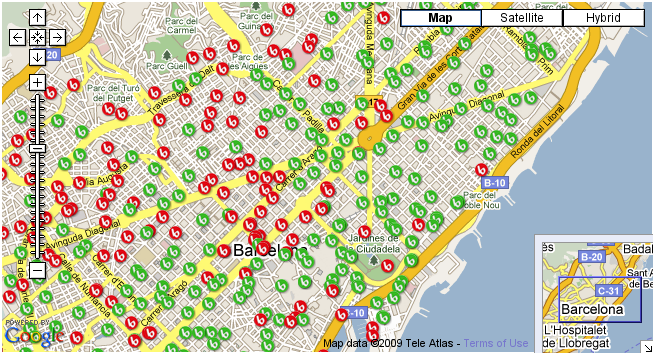
\includegraphics[width=\textwidth]{images/bicing_map.png}
\caption{Map of bicing stations in Barcelona -- red stations are without bikes}
\label{img:bicing_map}
\end{center}
\end{figure}

\section{Our task}



\end{document}          
